\section{Language of the Birds}

\begin{quotex}
And Solomon succeeded David. He said, ``O people, we were taught the \textbf{language of birds}, and we were given from everything. This is indeed a real blessing." \flright{\emph{Quran} 27:16}

\end{quotex}

\begin{wrapfigure}{rt}{.3\textwidth}
 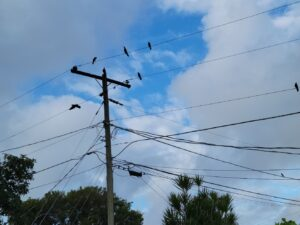
\includegraphics[scale=.5]{a20220508LanguageoftheBirds-img001.jpg} 
\end{wrapfigure}

\textbf{Rene Guenon} showed that the \textit{Language of the Birds}\footnote{\url{https://www.gornahoor.net/library/The_Language_of_the_Birds.pdf}} refers to communication with the higher states of the being. The Birds are symbols of the angels, or to be precise, of the higher states of being. A symbol is much deeper than an allegory. An allegory is a mechanical operation, just transposing one set of ideas to another on the same plane of existence. A symbol reaches into higher planes; it says something that could not be said any other way. Its secret is revealed in different ways for different traditions that refer to the language of the birds.

\paragraph{Secret Language}
In the sacred sciences like alchemy and magic, the Language of the Birds was a secret and perfect language, providing the key to perfect knowledge. John Dee made the association explicit: the Enochian language received from the angels was also the Language of the Birds.

\paragraph{Immortality}
Sigfried slew the dragon and tasted its flesh, which gave him the ability to learn the language of the birds. He smeared himself with dragon's blood, making his skin invulnerable, that is to say, he gained immortality. Guenon explains the symbolism:

\begin{quotex}
Victory over the dragon has, as its immediate consequence, the conquest of immortality, which is represented by some object the approach to which is guarded by the dragon; and this conquest essentially implies the reintegration into the center of the human state, that is, into the point where communication is established with the higher states of the being. 

\end{quotex}
\paragraph{Manifesting Possibilities}
\begin{quotex}
The Kingdom of Heaven is like a grain of mustard seed which a man took and sowed in his field; it is the smallest of all seeds, but when it has grown it is the greatest of shrubs and becomes a tree, so that the birds of the air come and make nests in its branches. \flright{\textsc{Matt 13:31-32}}

\end{quotex}
Guenon explains the symbolism of the Kingdom of Heaven:

\begin{itemize}
\item The growing of the tree is the manifestation of possibilities 
\item The birds of the air represent the higher states of the being 
\end{itemize}
\paragraph{The Observer}
The \textit{Mundaka Upanishad}\footnote{\url{https://www.wisdomlib.org/hinduism/book/mundaka-upanishad-shankara-bhashya}} expresses the language in this passage:

\begin{quotex}
Two birds, inseparably united companions, dwell in the same tree; the one eats of the fruit of the tree, while the other looks on without eating. \flright{\emph{Mundaka Upanishad} \textsc{iii.1}}

\end{quotex}
\begin{itemize}
\item The first bird is jivatma, who is involved in the realm of action. 
\item The second bird is the unconditioned Self, which observes 
\end{itemize}
\paragraph{Spiritual Battle}
The combat between Garuda, the Eagle, and the serpent Naga, symbolizes the spiritual battle between the Devas and the Asuras.

\paragraph{Angels}
How then can we understand the angelic language? \textbf{Pavel Florensky}, in \textit{The Meaning of Idealism}, clears up the relationship between the symbol and reality. The religious symbolism of the most ancient religions comes to life when we view it in the light of the fourth dimension. Those stuck in the world of three dimensions cannot understand the symbols. Florensky explains:

\begin{quotex}
Ideas, the Mothers of all existing things, live in the depth direction of our three-dimensional world, and therefore all speech regarding them remain nothing more the ``the jabbering gibberish of the Parcae".

\end{quotex}
There is, therefore, no transcendent vantage point to ``see" them, apart from the ``birds eye view". Things seem to be what they appear to be, but we miss the intelligence, the \emph{genii}, behind them. That is, we can't see the genus or archetype of the thing. Otherwise, we would experience them like this:

\begin{quotex}
[The ideas] are not images of gods but are the very consciousness of gods and demons appearing to initiates in the mysteries. Here we have gained entrance into the holy of holies of Plato's philosophy, where eidos and idea become concrete and full of life as well as transcendent.

\end{quotex}
Since the angels are pure intelligences, they are experienced in the Intellect, the higher thinking faculty. They are the source of the higher gnosis that we experience, i.e., the superconscious; the demons are the source of lower thoughts arising from the subconscious.

The higher that the angel is in the hierarchy, the more he can be understood in fewer thoughts. There is a constant battle against the chaos of the serpent. If the inner chaos is stilled, then, and only then, can the Language of the Birds be understood.


\hfill

\begin{quotex}
I think silence and the prolongation of sound is the same thing in terms of space. The only difference is that there is either the presence or absence of sound. More important is whether the space is ``living" or not. Our [Japanese] sense of time and space is different from that of the West. For example, in the Shinto religion, there is the term `imanaka' which is not just the present moment which lies between the stretch of past eternity and future immortality, but also the manifestation of the moment of all time which is multi-layered and multi-dimensional …. I would like it if the listener could abandon all previous conceptions of time and experience a new sense of time presented in this music as if eternal time can be lived in a single moment. \flright{\textsc{Somei Satoh}}

\end{quotex}

\url{https://www.youtube.com/watch?v=EE9V9TbPCBQ}


\flrightit{Posted on 2022-05-08 by Cologero }

\begin{center}* * *\end{center}

\begin{footnotesize}\begin{sffamily}



\texttt{Balder on 2022-05-16 at 13:55 said: }

I started thinking that could perhaps Odin's eagle and the hawk Vedfolnir play the same role as those birds mentioned in the Mundaka Upanishad? The hawk Vedfolnir is said to sit between the eyes of the unnamed eagle, and they both perch on top of the Yggdrasil. I find it difficult to interpret the hawk between the eyes of the eagle, but it might say the same thing the relationship between the two birds, namely Atma and jivatma. The eagle has been associated with Jupiter which I relate to Atma, but the hawk Vedfolnir doesn't seem to have any (traditionally atttested) planetary correspondence. This might be a procrustean attempt, but scholars have yet speculated that the Norse cosmology would have been influenced by the cosmologies of the East, and I think it is well attested that there is an Indo-European connection going back to pre-history.

I have enjoyed this spring time quite a lot by sitting in my balcony and listening to the singing of birds. I have made a habit to draw a weekly rune, and yesterday it was Algiz / Elhaz which is connected with swans, and in the night I listened to the sound of swans migrating back to the North for summer.


\end{sffamily}\end{footnotesize}
